\chapter{Scénarios d’intrusion (5 cas)}
\label{chap:chap_3}

\subsection{Scénario 1 — ICMP (ping)}
\textbf{Objectif :} Vérifier la capacité de l'IDS à détecter du trafic ICMP (ping).

\textbf{Justification :} Le ping est une méthode basique de reconnaissance utilisée pour confirmer la présence d'hôtes. Il s'agit d'un test simple permettant de valider la chaîne de détection (Suricata → syslog-ng → Elasticsearch → Kibana).

\textbf{Règle utilisée :}
\begin{lstlisting}[style=bashstyle]
alert icmp any any -> any any (msg:"ICMP test detected"; sid:1000001; rev:1;)
\end{lstlisting}

\textbf{Procédure :} exécution de \texttt{ping -c 6 8.8.8.8} depuis la VM.

\begin{figure}[H]
    \centering
    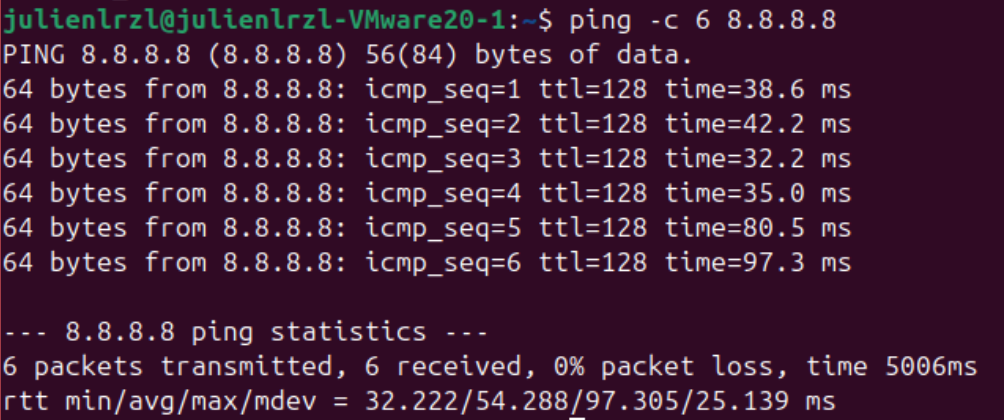
\includegraphics[width=0.9\linewidth]{assets/figures/scen1_ping_cmd.png}
    \caption{Commande \texttt{ping} exécutée dans le terminal (génération du trafic ICMP).}
    \label{fig:scen1_ping_cmd}
\end{figure}

\textbf{Preuves :} la figure \ref{fig:scen1_fastlog} montre l'entrée correspondante dans \path{/var/log/suricata/fast.log} et la figure \ref{fig:scen1_kibana} présente l'alerte remontée dans Kibana Discover.

\begin{figure}[H]
    \centering
    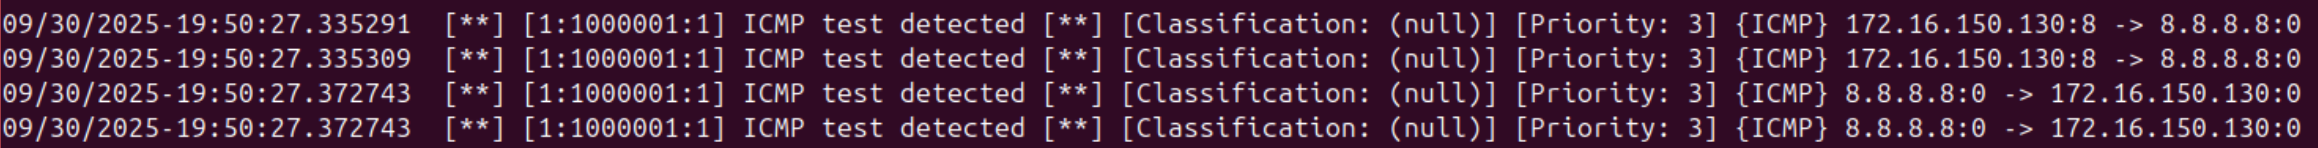
\includegraphics[width=0.9\linewidth]{assets/figures/scen1_fastlog.png}
    \caption{Alerte ICMP détectée par Suricata (extrait de fast.log).}
    \label{fig:scen1_fastlog}
\end{figure}

\begin{figure}[H]
    \centering
    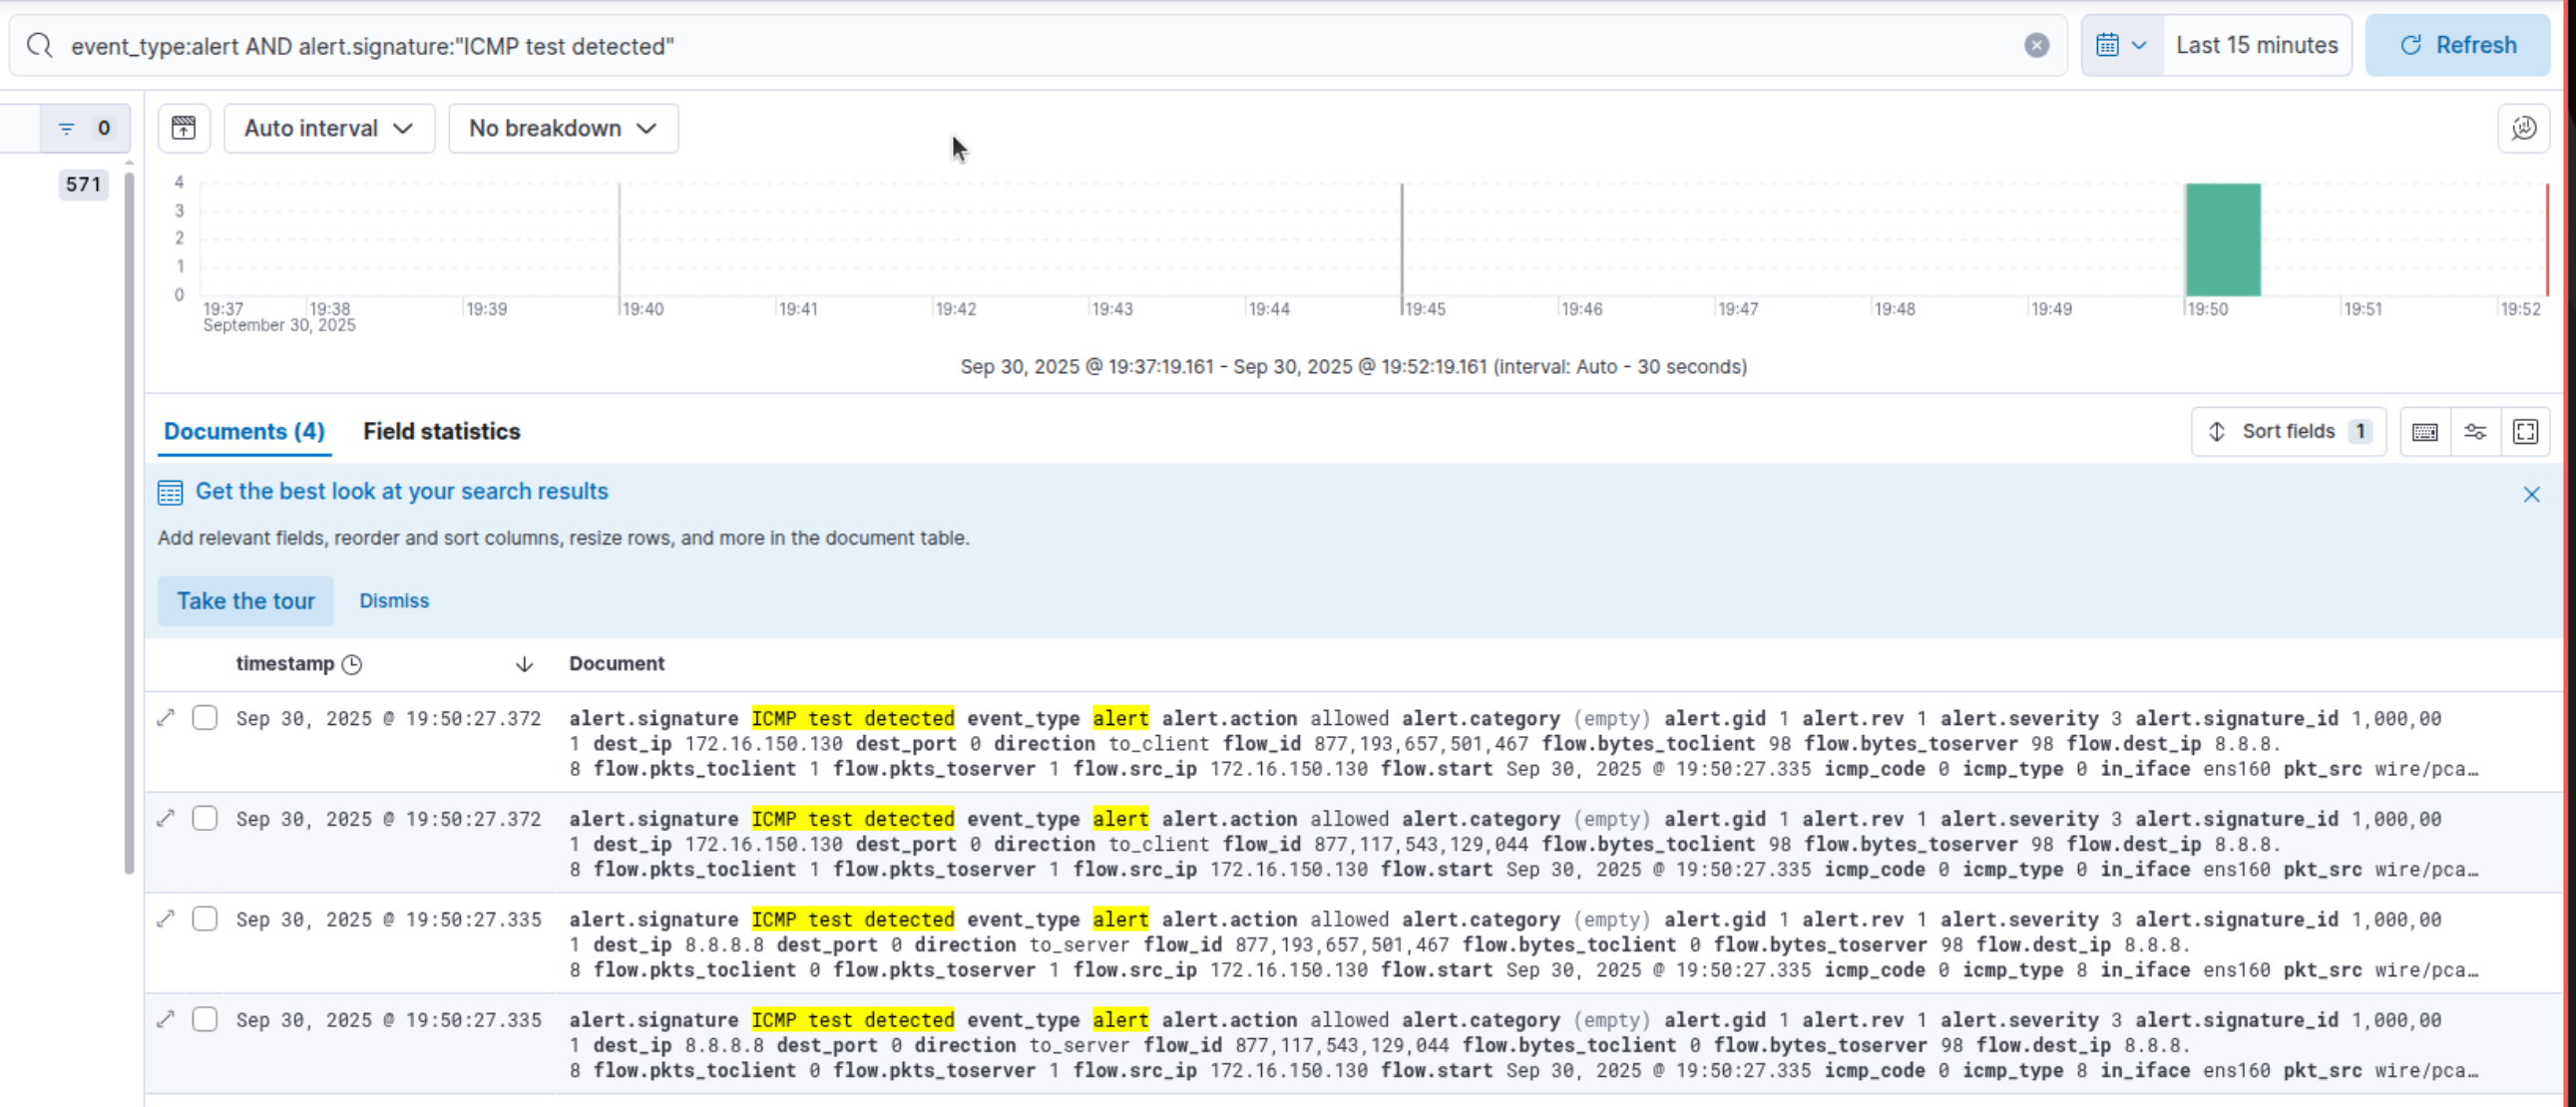
\includegraphics[width=0.9\linewidth]{assets/figures/scen1_kibana_discover.png}
    \caption{Alerte ICMP visible dans Kibana Discover.}
    \label{fig:scen1_kibana}
\end{figure}

\textbf{Utilité en conditions réelles :} le ping est utilisé par les administrateurs pour vérifier la disponibilité d’un hôte, mais aussi par des attaquants pour repérer des cibles actives lors de la phase de reconnaissance ; détecter et alerter sur ces requêtes permet de repérer des scans précoces et d'initier des mesures de durcissement ou de surveillance.

\clearpage
\subsection{Scénario 2 — Reconnaissance : scan Nmap}
\textbf{Objectif :} Détecter une activité de reconnaissance réseau (scan de ports).

\textbf{Justification :} Les scans de ports font partie des premières étapes d'une attaque : un attaquant cherche quels services sont exposés. Détecter ces scans permet d'anticiper des tentatives d'exploitation ultérieures.

\textbf{Règle utilisée :}
\begin{verbatim}
alert tcp any any -> any any (msg:"TCP portscan";
    threshold:type limit, track by_src, count 20, seconds 10;
    sid:1000004; rev:1;)
\end{verbatim}

\textbf{Procédure :} exécution d'un scan local depuis la VM :
\begin{verbatim}
sudo nmap -sS --top-ports 100 127.0.0.1
\end{verbatim}

\begin{figure}[H]
    \centering
    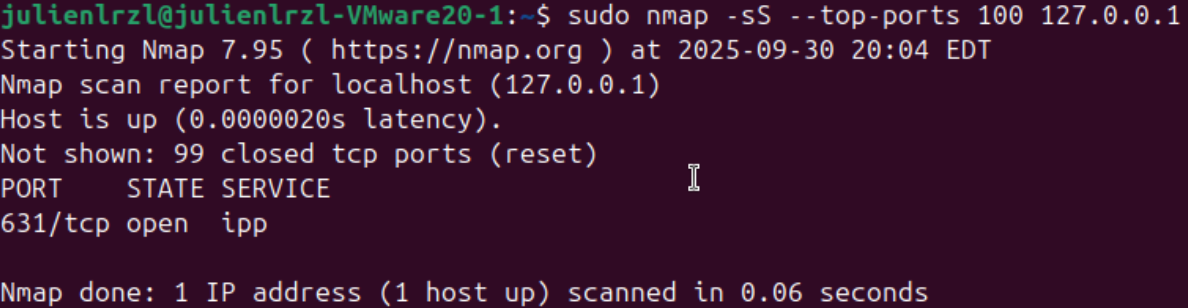
\includegraphics[width=0.9\linewidth]{assets/figures/scen2_nmap_cmd.png}
    \caption{Commande Nmap exécutée pour générer l'activité de reconnaissance.}
    \label{fig:scen2_nmap}
\end{figure}

\textbf{Preuves :} la figure \ref{fig:scen2_fastlog} montre l'entrée d'alerte correspondante dans \path{/var/log/suricata/fast.log} et la figure \ref{fig:scen2_kibana} présente les événements indexés et visibles dans Kibana Discover.

\begin{figure}[H]
    \centering
    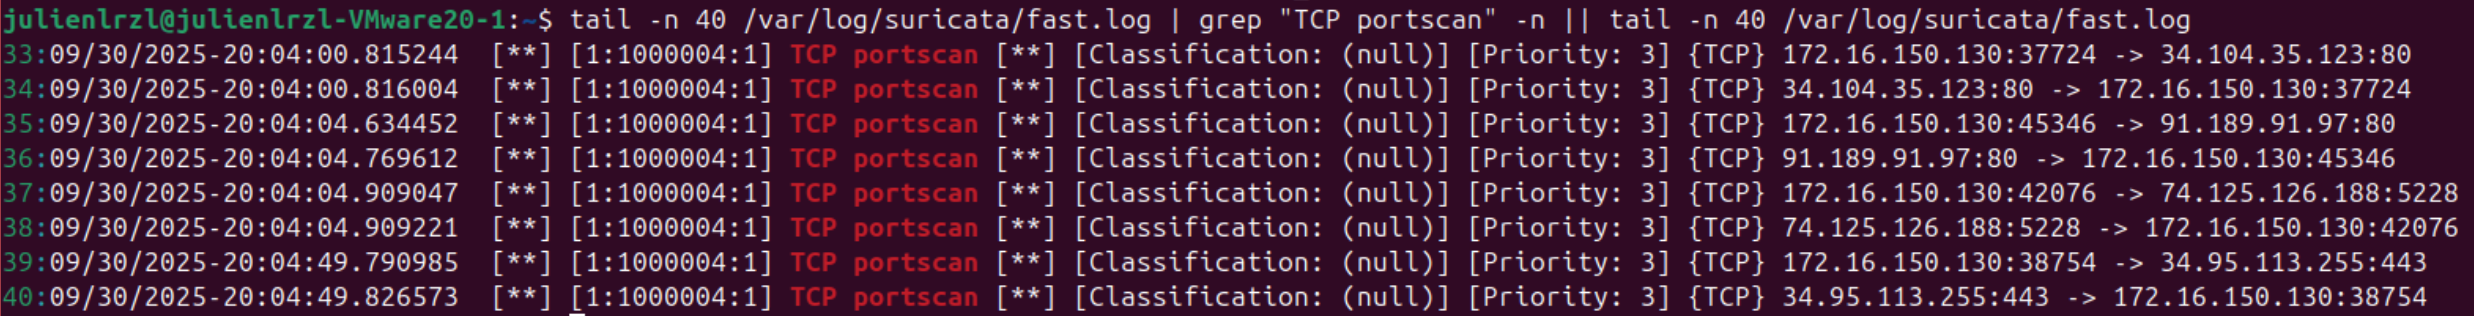
\includegraphics[width=0.9\linewidth]{assets/figures/scen2_fastlog.png}
    \caption{Alerte de type \texttt{TCP portscan} détectée par Suricata (extrait de fast.log).}
    \label{fig:scen2_fastlog}
\end{figure}

\begin{figure}[H]
    \centering
    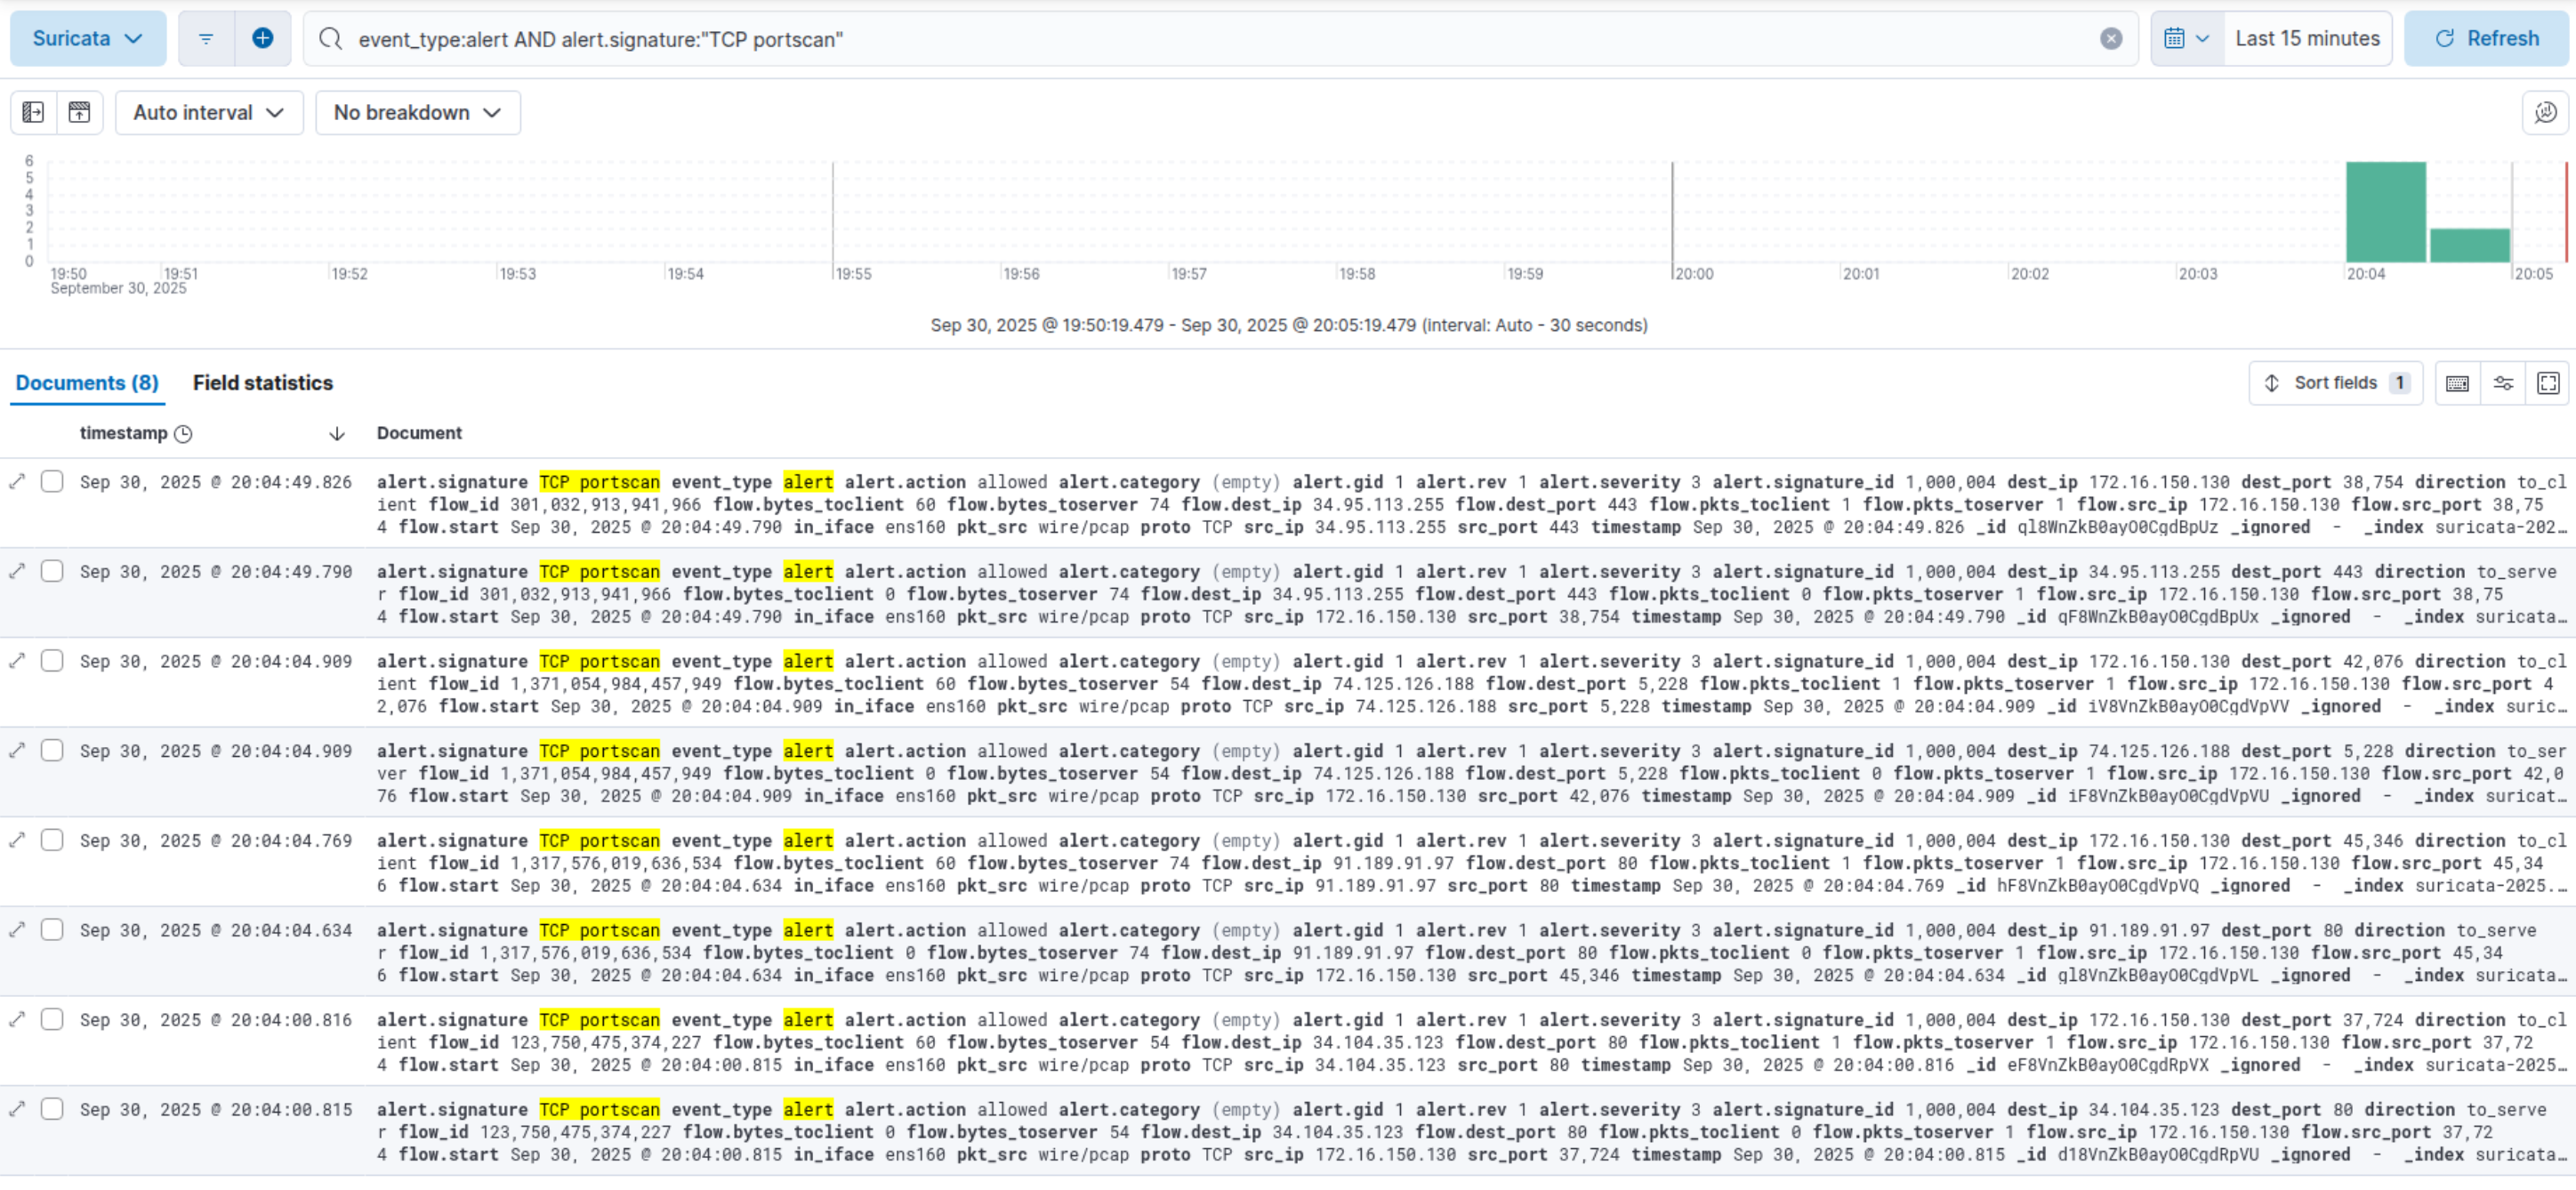
\includegraphics[width=0.9\linewidth]{assets/figures/scen2_kibana_discover.png}
    \caption{Evénements \texttt{TCP portscan} visibles dans Kibana Discover.}
    \label{fig:scen2_kibana}
\end{figure}

\textbf{Analyse :} L'alerte confirme la détection d'une activité de reconnaissance. En environnement réel, la détection précoce d'un scan permet de déclencher des contre-mesures (blocage d'IP, investigation, enrichissement des logs).

\clearpage
\subsection{Scénario 3 — Tentatives SSH}
\textbf{Objectif :} Détecter des connexions SSH (et potentiellement des tentatives de brute-force).

\textbf{Justification :} Le protocole SSH est chiffré et ne peut pas être analysé en profondeur par l’IDS. Néanmoins, il est possible de détecter les tentatives de connexion sur le port 22, ainsi que des patterns anormaux de connexions répétées, ce qui peut indiquer une attaque par force brute.

\textbf{Règles utilisées :}
\begin{lstlisting}[style=bashstyle]
alert tcp $EXTERNAL_NET any -> $HOME_NET 22 (msg:"Possible SSH brute forcing!"; flags: S+; threshold: type both, track by_src, count 5, seconds 30; sid:10000001; rev: 1;)
\end{lstlisting}

\textbf{Procédure :} génération de connexions TCP vers le port 22 en boucle, simulant des tentatives répétées de connexion SSH :
\begin{verbatim}
for i in $(seq 1 10); do nc -vz 172.16.150.130 22; sleep 0.3; done
\end{verbatim}

\begin{figure}[H]
    \centering
    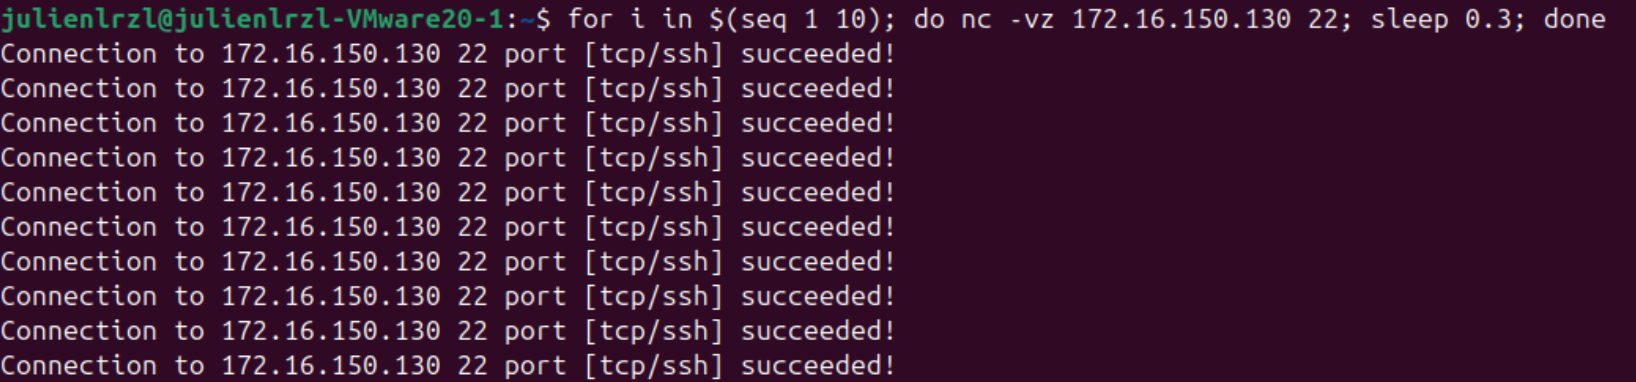
\includegraphics[width=0.9\linewidth]{assets/figures/scen3_nc_cmd.png}
    \caption{Commande \texttt{nc} utilisée pour simuler des connexions SSH répétées sur le port 22.}
    \label{fig:scen3_nc_cmd}
\end{figure}

\textbf{Preuves :} la figure \ref{fig:scen3_fastlog} montre l’entrée d’alerte dans \path{/var/log/suricata/fast.log} et la figure \ref{fig:scen3_kibana} présente l’événement visible dans Kibana Discover.

\begin{figure}[H]
    \centering
    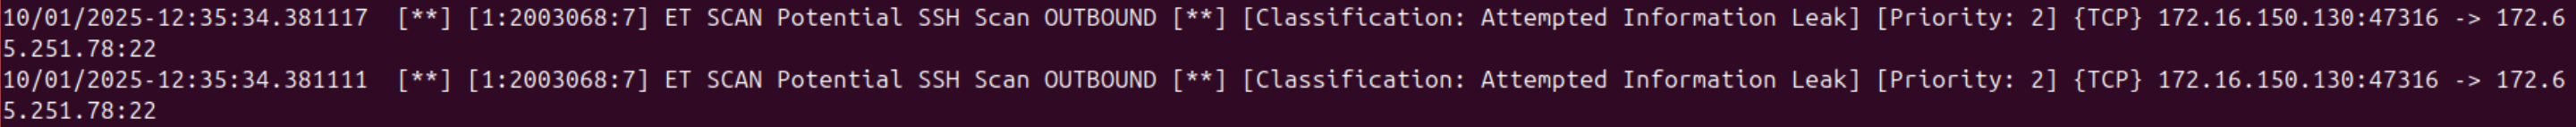
\includegraphics[width=0.9\linewidth]{assets/figures/scen3_fastlog.png}
    \caption{Alertes SSH détectées par Suricata (extrait de fast.log).}
    \label{fig:scen3_fastlog}
\end{figure}

\begin{figure}[H]
    \centering
    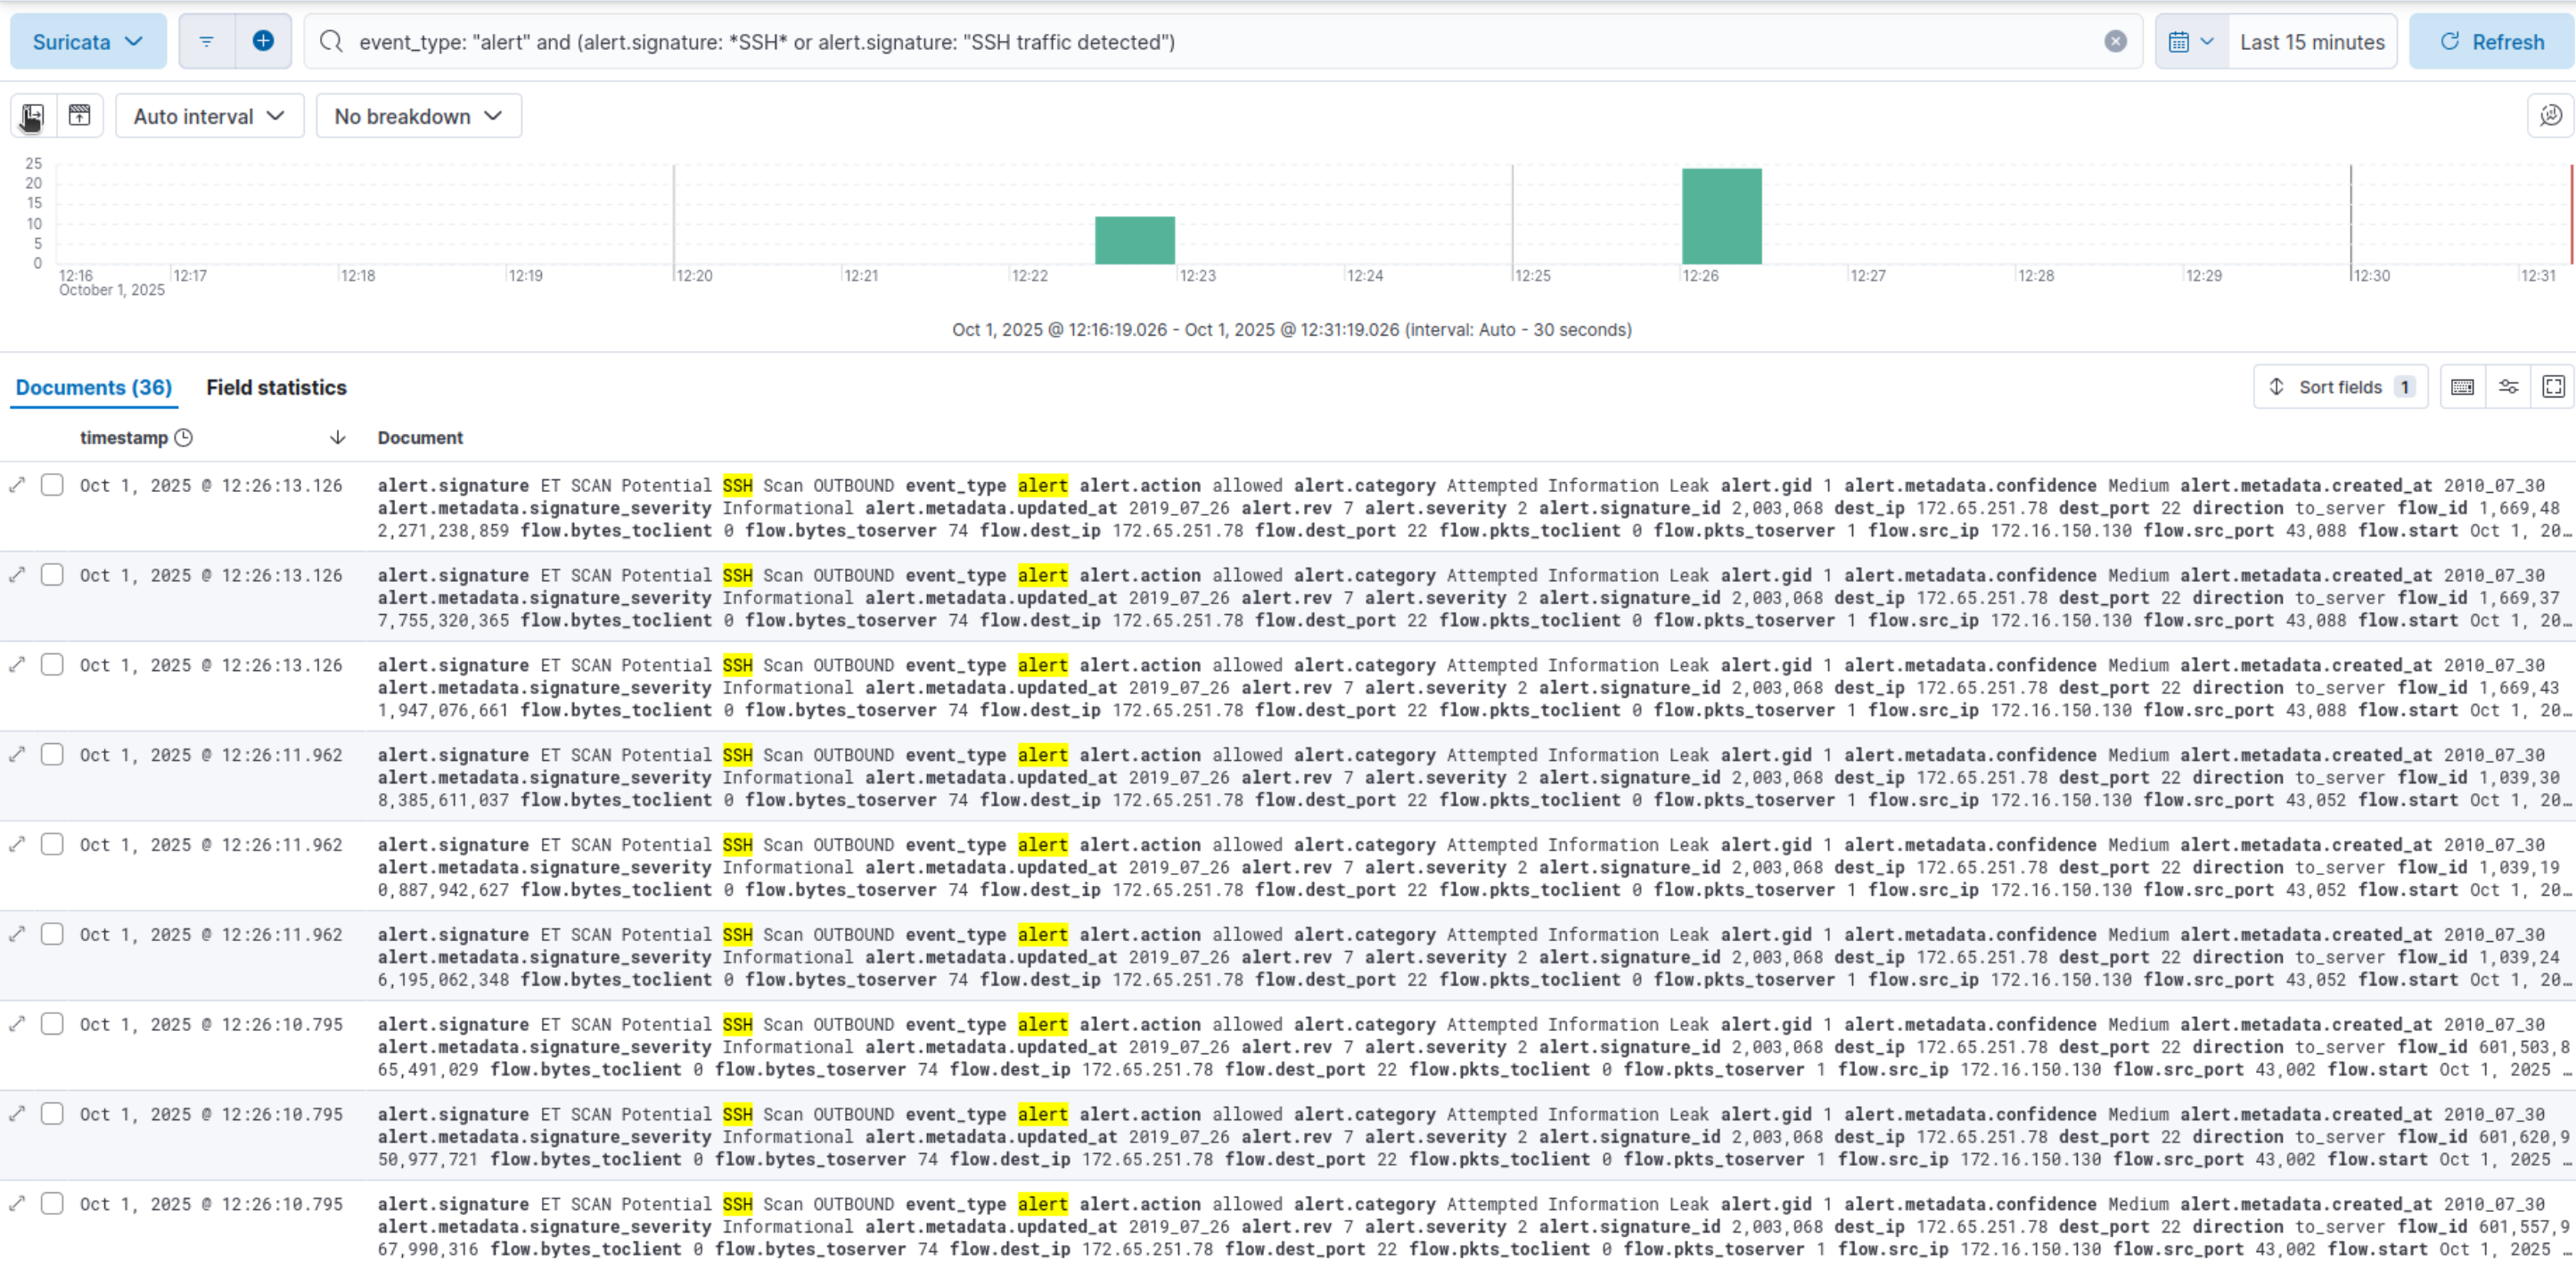
\includegraphics[width=0.9\linewidth]{assets/figures/scen3_kibana.png}
    \caption{Événements SSH détectés dans Kibana Discover.}
    \label{fig:scen3_kibana}
\end{figure}

\textbf{Analyse :}  
Les alertes confirment que Suricata détecte bien le trafic SSH sur le port 22.  
Dans un contexte réel, cela permet de repérer rapidement des tentatives suspectes (par exemple un outil d’attaque par dictionnaire). Même si le contenu SSH reste chiffré, la corrélation entre fréquence et volume des connexions permet d’identifier un comportement anormal. Couplé aux logs système d’authentification (\path{/var/log/auth.log}), cela permet de confirmer une tentative de brute-force.

\clearpage
\subsection{Scénario 4 — Fuzzing web (volume élevé)}
\textbf{Objectif :} Détecter un volume anormalement élevé de requêtes HTTP provenant d'une même source (possible fuzzing / scanner web).

\textbf{Règle utilisée :}
\begin{lstlisting}[style=bashstyle]
alert http any any -> any any (
  msg:"WEB-FUZZ - High HTTP request rate from source (possible fuzzing)";
  flow:to_server,established;
  detection_filter: track by_src, count 100, seconds 60;
  sid:1002001; rev:1; classtype:attempted-recon; priority:2;
)
\end{lstlisting}

\textbf{Procédure :}
\begin{lstlisting}[style=bashstyle]
seq 1 200 | xargs -n1 -P20 -I{} curl -s -o /dev/null "http://172.16.150.130:5601/index.html"
\end{lstlisting}

\textbf{Preuves :} la figure \ref{fig:scen4_fastlog} montre l’alerte dans \path{/var/log/suricata/fast.log} et la figure \ref{fig:scen4_kibana_discover} l’événement indexé et visible dans Kibana Discover.

\begin{figure}[H]
    \centering
    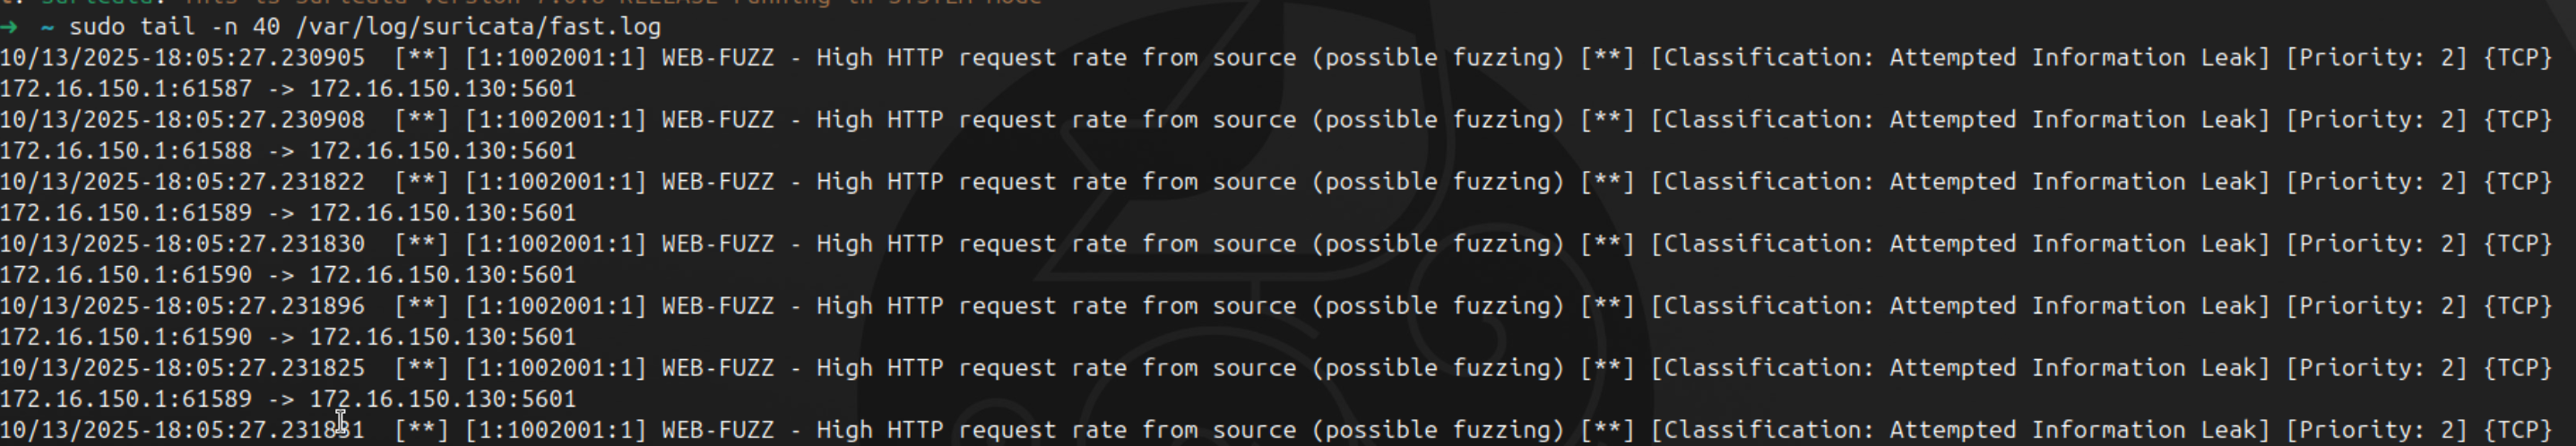
\includegraphics[width=0.9\linewidth]{assets/figures/scen4_fastlog.png}
    \caption{Alerte \texttt{WEB-FUZZ} détectée par Suricata (extrait de fast.log).}
    \label{fig:scen4_fastlog}
\end{figure}

\begin{figure}[H]
    \centering
    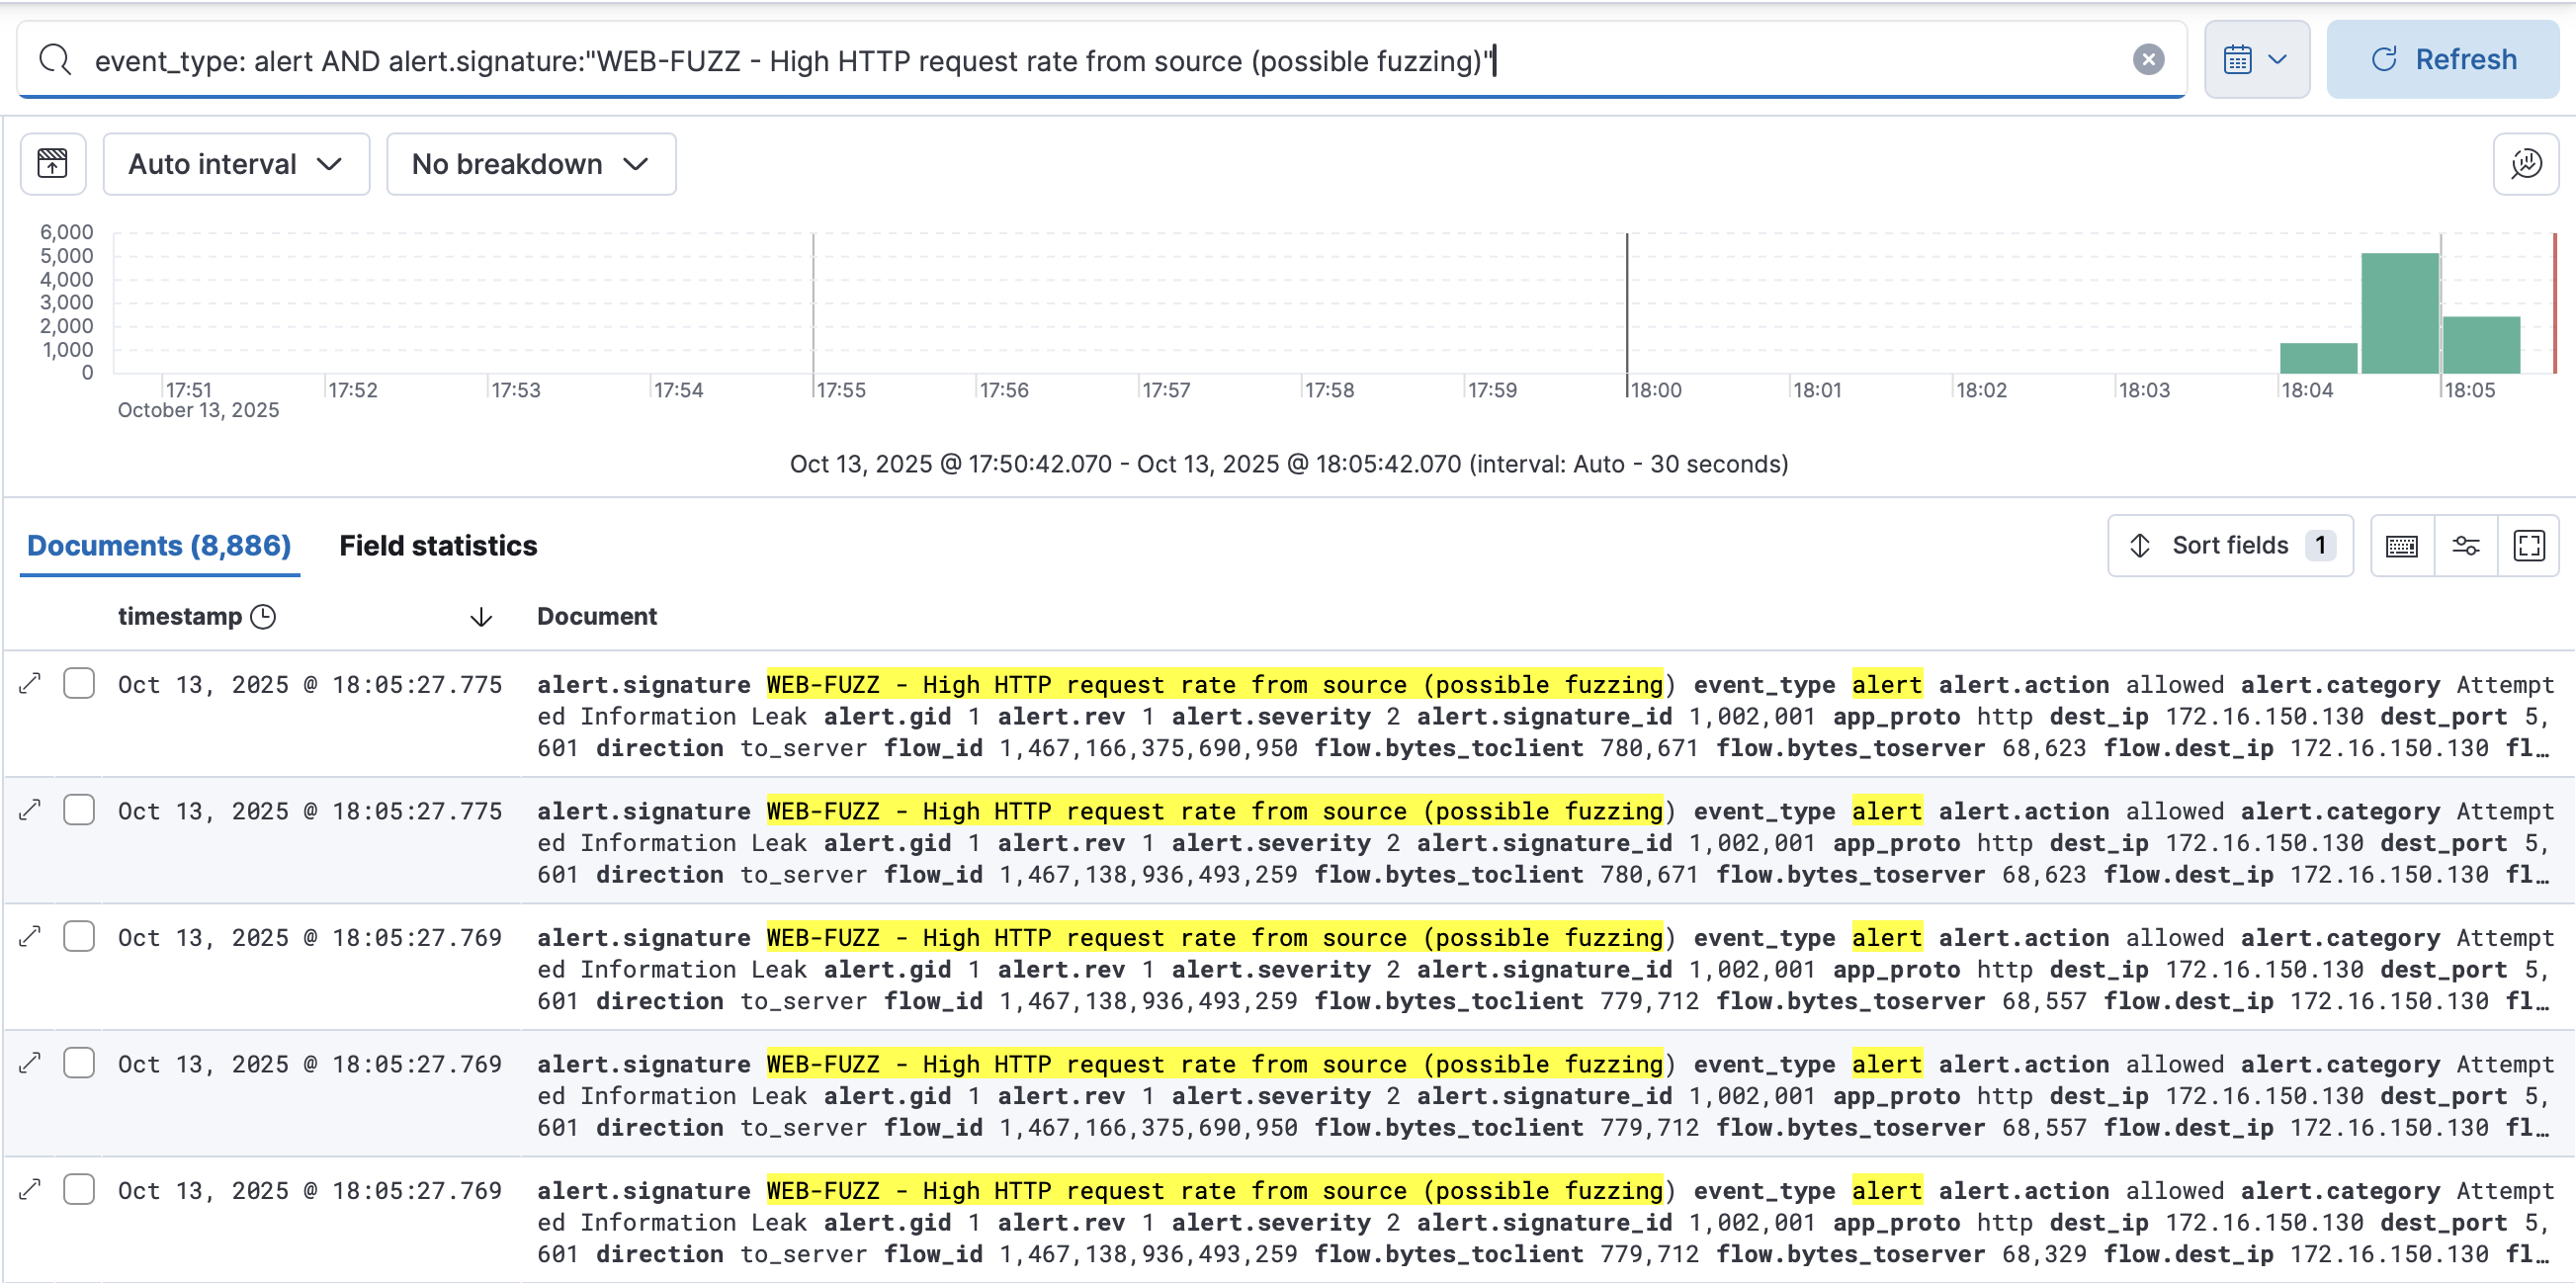
\includegraphics[width=0.9\linewidth]{assets/figures/scen4_kibana_discover.png}
    \caption{Evénement \texttt{WEB-FUZZ} indexé et visible dans Kibana Discover.}
    \label{fig:scen4_kibana_discover}
\end{figure}

\textbf{Analyse :} Cette règle est utile pour repérer des scans/fuzzing orientés web. En production, attention aux faux positifs (par ex. tests de charge légitimes) : corréler à des sources connues et ajuster seuils. Combiner cette règle avec des logs d’accès web et des systèmes de blocage automatique (Fail2Ban / WAF) améliore la réponse.

\clearpage
\subsection{Scénario 5 — FTP : tentative d'accès anonyme}
\textbf{Objectif :} Détecter une tentative d'accès FTP en mode anonyme (login \texttt{anonymous}), typique d’un accès public ou d’un test de découverte de services.

\textbf{Justification :} Les serveurs FTP mal configurés autorisant l'accès anonyme peuvent être utilisés pour exfiltrer ou déposer des fichiers. Détecter les tentatives \texttt{USER anonymous} permet d'identifier des services exposés ou des tests automatisés d'accès.

\textbf{Règle utilisée :}
\begin{lstlisting}[style=bashstyle]
alert tcp any any -> any 21 (msg:"FTP anonymous login attempt"; \
content:"USER anonymous"; nocase; sid:1003001; rev:1;)
\end{lstlisting}

\textbf{Procédure :} exécution de la commande FTP en mode anonyme depuis l'exterieur :
\begin{lstlisting}[style=bashstyle]
    nc -vz 172.16.150.130 21
\end{lstlisting}

\textbf{Preuves :} la figure \ref{fig:scen_ftp_fastlog} montre l’alerte dans \path{/var/log/suricata/fast.log} et la figure \ref{fig:scen_ftp_kibana} l’événement remonté dans Kibana Discover.

\begin{figure}[H]
    \centering
    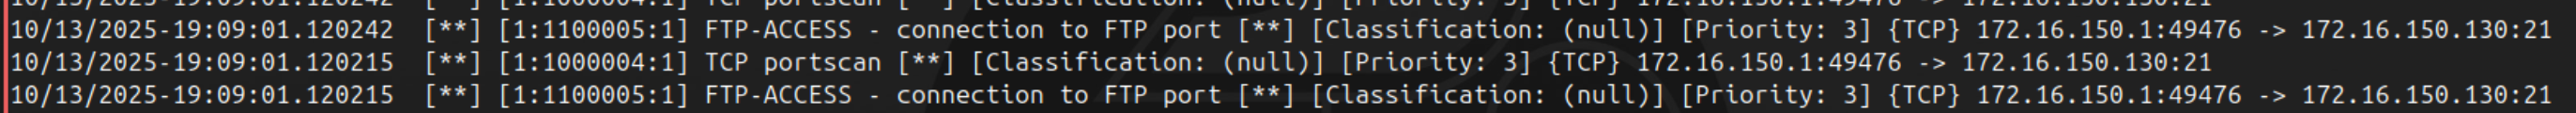
\includegraphics[width=0.9\linewidth]{assets/figures/scen_ftp_fastlog.png}
    \caption{Alerte \texttt{FTP anonymous login attempt} détectée par Suricata (extrait de fast.log).}
    \label{fig:scen_ftp_fastlog}
\end{figure}

\begin{figure}[H]
    \centering
    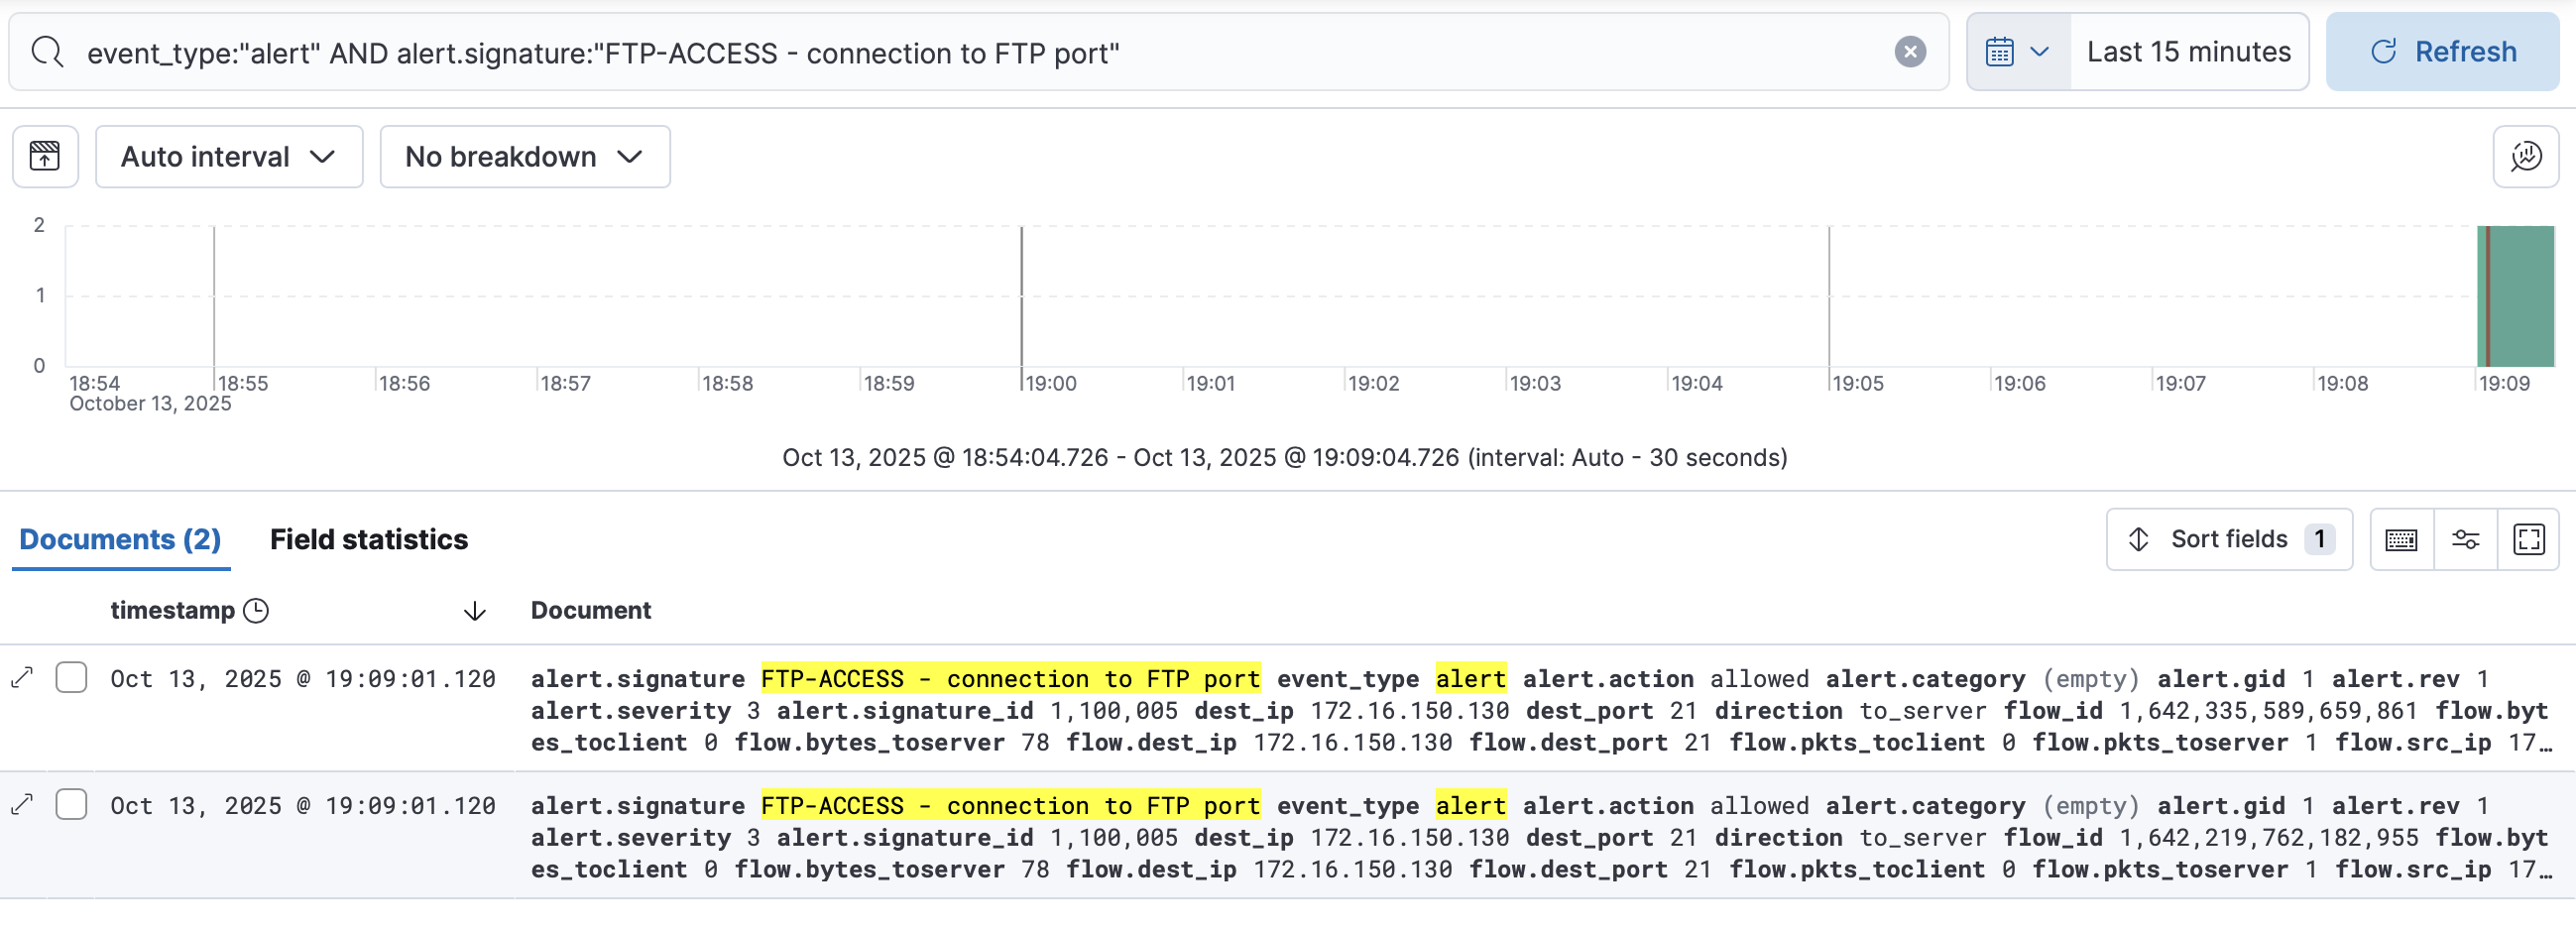
\includegraphics[width=0.9\linewidth]{assets/figures/scen_ftp_kibana.png}
    \caption{Evénement FTP anonyme visible dans Kibana Discover.}
    \label{fig:scen_ftp_kibana}
\end{figure}

\textbf{Analyse :}  
La règle détecte l’envoi explicite du login \texttt{USER anonymous}. En production, il faudra :
\begin{itemize}
  \item réduire les faux positifs en corrélant avec les logs du service FTP (\path{/var/log/vsftpd.log} ou \path{/var/log/auth.log}) ;
  \item éventuellement améliorer la règle (par exemple détection de \texttt{PASS} faibles, détection de transferts après login anonyme, ou surveillance d'un grand nombre de fichiers transférés) ;
  \item si nécessaire, bloquer automatiquement l’IP source (via firewall / fail2ban) ou désactiver l’anonymous sur le serveur.
\end{itemize}